\chapter{Les calculs parallèles}

Mon apprentissage du calcul parallèle s'est fait en parallélisant un programme séquentiel calculant le produit de deux matrices à l'aide d'OpenMP \cite{ref1}. Avant d'expliquer comment fonctionne OpenMP et son utilisation, un bref rappel sur le calcul matriciel s'impose afin de comprendre en quoi il constitue l'exemple parfait pour aborder les calculs parallèles. 

\section{Pourquoi choisir le calcul matriciel}
Notons A et B deux matrices carrées de taille n dont nous souhaitons faire le produit. Notons C la matrice résultat, elle est également carrée de taille n. 
\begin{equation*}
\begin{pmatrix}
	a_{1,1} & \cdots & & \cdots & a_{1,n} \\
	\vdots & & \vdots & &\vdots \\
	a_{i,1} & \cdots & a_{i,k} & \cdots & a_{i,n} \\
	\vdots & & \vdots & & \vdots \\
	a_{n,1} & \cdots & & \cdots & a_{n,n} 
\end{pmatrix} 
\begin{pmatrix}
	b_{1,1} & \cdots & b_{1,j} & \cdots & b_{1,n} \\
	\vdots & & \vdots & &\vdots \\
	  & \cdots & b_{k,j} & \cdots &   \\
	\vdots & & \vdots & & \vdots \\
	b_{n,1} & \cdots & b_{n,j} & \cdots & b_{n,n} 
\end{pmatrix}
=
\begin{pmatrix}
	c_{1,1} & \cdots & & \cdots & c_{1,n} \\
	\vdots & & \vdots & &\vdots \\
	c_{i,1} & \cdots & c_{i,j} & \cdots & c_{i,n} \\
	\vdots & & \vdots & & \vdots \\
	c_{n,1} & \cdots & & \cdots & c_{n,n} 
\end{pmatrix}
\end{equation*}

Le calcul de l'élément (i,j) de la matrice C est réalisé à l'aide de la \hyperref[formule:3.1]{Formule 3.1}.
\begin{equation}
\large{C_{i,j} = \sum_{k=1}^{n} A_{i,k}*B_{k,j}} \label{formule:3.1}
\end{equation}

Nous voyons ici que l'élément (i,j) calculé est indépendant au niveau des calculs, de tous les autres éléments de la matrice résultat. Ainsi, l'entité réalisant le produit, que ce soit l'ordinateur ou un être humain, pourra calculer les éléments dans l'ordre qu'il souhaite sans que cela ait un effet sur la validité du résultat. C'est cela qui rend le produit matriciel intéressant pour appréhender le parallélisme. En effet, l'ordinateur, s'il dispose des ressources nécessaires, pourra calculer simultanément plusieurs éléments de la matrice résultat en assignant les calculs à plusieurs de ses processeurs plutôt que d'en laisser un seul effectuer l'ensemble des calculs.

\section{OpenMP}

OpenMP est une interface de programmation applicative permettant de paralléliser des programmes écrits en langage Fortran ou bien en C/C++. Il s'utilise à l'aide de directives destinées au compilateur que le programmeur ajoute à son programme séquentiel afin de distribuer le travail entre les différents processeurs ou coeurs en spécifiant quelles données doivent être partagées ou privées. Ceci rend son utilisation et son apprentissage extrêmement simple. Un exemple d'utilisation est donné dans la \hyperref[figure:3.1]{Figure 3.1} .    
\begin{figure}[hb]

	\begin{center}
	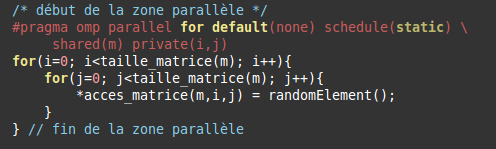
\includegraphics[scale=0.7]{exemple_OpenMP.png} 
	\end{center}
	\caption{Exemple d'utilisation d'un directive OpenMP}
	\label{figure:3.1}

\end{figure}
Dans cette figure nous pouvons voir comment est parallélisée une zone d'un programme à l'aide d'OpenMP. La directive "\#pragma omp parallel" permet d'indiquer au compilateur qu'il faut qu'une zone parallèle soit créée. L'ajout du "for" permet d'indiquer que la zone à paralléliser sera une boucle \textbf{For}. S'ajoutent ensuite différentes clauses qui permettent entre autre de choisir de quelle manière sera distribué le travail entre les différents threads ou encore combien de threads devront être utilisés. Enfin, le programmeur peut indiquer au compilateur quelles données seront partagées par les threads et celles dont chaque thread devra posséder une copie qu'il manipulera ensuite (le programmeur peut laisser le compilateur faire ce choix à sa place mais cela est vivement déconseillé). Une directive complète sera analysée plus en détail plus loin dans le rapport. \\
 
Le plus compliqué reste en fait d'identifier les zones d'un programme propices à une exécution parallèle. Ainsi, le programmeur devra de temps en temps changer un de ses algorithmes afin d'optimiser son programme pour le parallélisme.  


\section{Premiers algorithmes et résultats}

J'ai choisi de manipuler uniquement des matrices représentées en mémoire par des tableaux monodimensionnels. Dans ce type de structure les lignes de la matrice sont stockées les unes après les autres en mémoire. Ceci améliore grandement la localité de nos données tout en évitant de nombreuses indirections. \\

J'ai commencé par implémenter l'algorithme naïf permettant d'effectuer le produit de deux matrices (carrées dans mon cas). Celui-ci est donné en \hyperref[figure:3.2]{Figure 3.2} . Paralléliser ce programme fut relativement simple (c'est d'ailleurs la version parallèle qui est présentée).

Pour plus d'informations, se référer à la documentation d'OpenMP\footnote{\url{http://openmp.org/wp/openmp-specifications/}}

\begin{figure}[ht]

	\begin{center}
	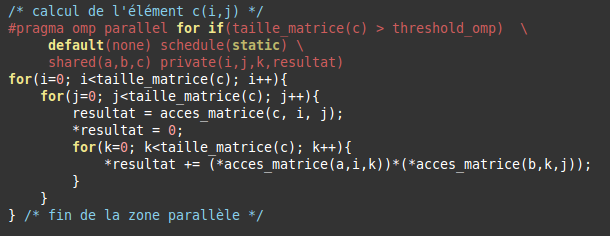
\includegraphics[scale=0.6]{algo_naif.png} 
	\end{center}
	\caption{Implémentation en C de l'algorithme naïf du produit matriciel}
	\label{figure:3.2}

\end{figure}

La \hyperref[figure:3.3]{Figure 3.3} présente une analyse des premiers résultats obtenus. Une série comparative des temps d'exécutions sur de très petites matrices lorsque les calculs sont réalisés en parallèle avec 8 threads et lorsqu'ils sont réalisés séquentiellement par 1 seul thread. 

\begin{figure}

	\begin{center}
	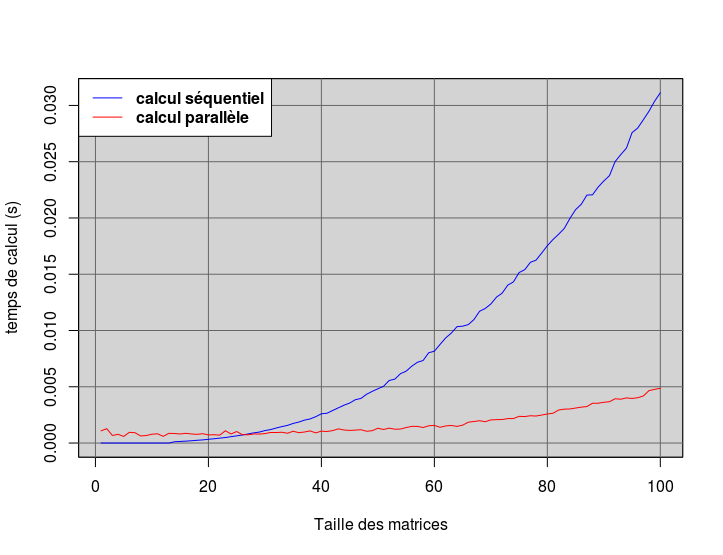
\includegraphics[scale=0.6]{premiers_resultats.png} 
	\end{center}
	\caption{Comparaison des temps de calculs sur des matrices de tailles 1x1 à 128x128}
	\label{figure:3.3}

\end{figure}

S'en est suivi une série de mesures permettant de mesurer l'accélération obtenue en utilisant les calculs parallèles en fonction du nombre de threads. 

Comme nous pouvons le voir dans cet algorithme, la matrice A est parcourue séquentiellement à l'inverse de la matrice B ce qui, comme nous l'avons vu dans la \hyperref[Section:2.2]{Section 2.2}, n'est pas une bonne chose. Pour chaque donnée de la matrice B requise par l'un des processeurs, et en considérant que nos matrices soient suffisamment grandes, une ligne de cache devra être extraite de la mémoire principale. De plus, cette dernière sera probablement évincée du cache avant d'être réutilisée. S'en suivent des performances médiocres. \\

L'une des façons d'améliorer les performances dans ce cas est de transposer la matrice B avant de réaliser les calculs afin de pouvoir la parcourir séquentiellement et donc d'utiliser les données présentes dans la mémoire cache. La \hyperref[formule:3.2]{Formule 3.2} donne le calcul de l'élément C(i,j) dans le cas où la transposée de la matrice B est utilisée.
\begin{equation}
\large{C_{i,j} = \sum_{k=1}^{n} A_{i,k}*{}^t \! B_{j,k}} \label{formule:3.2}
\end{equation}
 La \hyperref[figure:3.3]{Figure 3.4} présente une comparaison des temps de calculs avec les deux algorithmes en utilisant 8 threads. 

\begin{figure}[hb]

	\begin{center}
	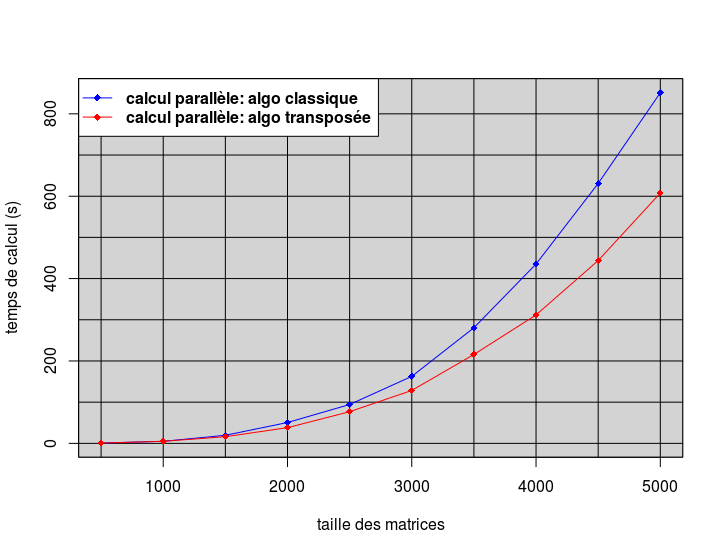
\includegraphics[scale=0.7]{para_transposee_500_5000.png} 
	\end{center}
	\caption{Comparaison des temps de calculs en fonction des algorithmes et de la taille des matrices}
	\label{figure:3.4}

\end{figure}

Nous pouvons voir que le surcoût d'opérations lié à la transposition de la matrice B est rapidement compensé par une bien meilleure utilisation du cache lors des calculs. Néanmoins, ces résultats restent peu satisfaisants car ils laissent présager des temps de calcul très longs pour de grosses matrices\footnote{des matrices dont la taille est inférieure à 10 000 sont considérées comme de petites matrices par les scientifiques étudiant les calculs parallèles}, la courbe des temps d'exécutions étant cubique! \\
C'est ici qu'une bonne utilisation de la mémoire peut nous faire gagner de nombreuses secondes. L'idée va être de séparer nos matrices en plusieurs blocs de tailles égales 


